\chapter{Algoritmos de raíz cuadrada}

\index{algoritmo de raíz cuadrada}

Un \key{algoritmo de raíz cuadrada} es un algoritmo
que tiene una raíz cuadrada en su complejidad temporal.
Una raíz cuadrada puede ser vista como un ''logaritmo del pobre'':
la complejidad $O(\sqrt n)$ es mejor que $O(n)$
pero peor que $O(\log n)$.
En cualquier caso, muchos algoritmos de raíz cuadrada son rápidos y utilizables en la práctica.

Como ejemplo, consideremos el problema de
crear una estructura de datos que soporte
dos operaciones en un arreglo:
modificar un elemento en una posición dada
y calcular la suma de los elementos en el rango dado.
Anteriormente hemos resuelto el problema utilizando
árboles binarios indexados y segmentados,
que soportan ambas operaciones en tiempo $O(\log n)$.
Sin embargo, ahora resolveremos el problema
de otra manera usando una estructura de raíz cuadrada
que nos permite modificar elementos en tiempo $O(1)$
y calcular sumas en tiempo $O(\sqrt n)$.

La idea es dividir el arreglo en \emph{bloques}
de tamaño $\sqrt n$ de manera que cada bloque contenga
la suma de los elementos dentro del bloque.
Por ejemplo, un arreglo de 16 elementos será
dividido en bloques de 4 elementos como sigue:

\begin{center}
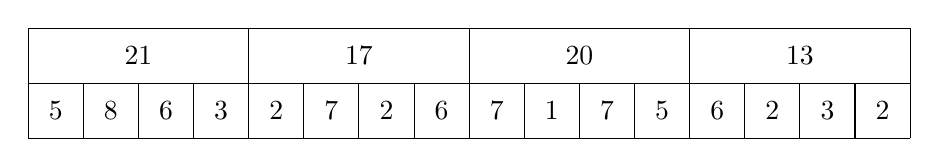
\begin{tikzpicture}[scale=0.7]
\draw (0,0) grid (16,1);

\draw (0,1) rectangle (4,2);
\draw (4,1) rectangle (8,2);
\draw (8,1) rectangle (12,2);
\draw (12,1) rectangle (16,2);

\node at (0.5, 0.5) {5};
\node at (1.5, 0.5) {8};
\node at (2.5, 0.5) {6};
\node at (3.5, 0.5) {3};
\node at (4.5, 0.5) {2};
\node at (5.5, 0.5) {7};
\node at (6.5, 0.5) {2};
\node at (7.5, 0.5) {6};
\node at (8.5, 0.5) {7};
\node at (9.5, 0.5) {1};
\node at (10.5, 0.5) {7};
\node at (11.5, 0.5) {5};
\node at (12.5, 0.5) {6};
\node at (13.5, 0.5) {2};
\node at (14.5, 0.5) {3};
\node at (15.5, 0.5) {2};

\node at (2, 1.5) {21};
\node at (6, 1.5) {17};
\node at (10, 1.5) {20};
\node at (14, 1.5) {13};

\end{tikzpicture}
\end{center}

En esta estructura,
es fácil modificar los elementos del arreglo,
porque solo es necesario actualizar
la suma de un solo bloque
después de cada modificación,
lo cual puede hacerse en tiempo $O(1)$.
Por ejemplo, la siguiente imagen muestra
cómo cambia el valor de un elemento y
la suma del bloque correspondiente:

\begin{center}
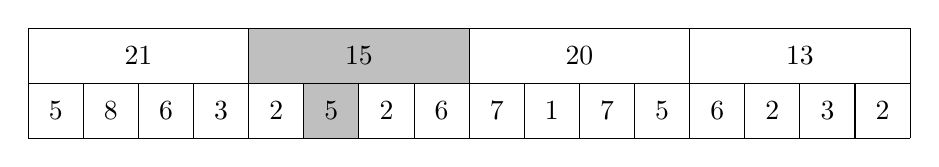
\begin{tikzpicture}[scale=0.7]
\fill[color=lightgray] (5,0) rectangle (6,1);
\draw (0,0) grid (16,1);

\fill[color=lightgray] (4,1) rectangle (8,2);
\draw (0,1) rectangle (4,2);
\draw (4,1) rectangle (8,2);
\draw (8,1) rectangle (12,2);
\draw (12,1) rectangle (16,2);

\node at (0.5, 0.5) {5};
\node at (1.5, 0.5) {8};
\node at (2.5, 0.5) {6};
\node at (3.5, 0.5) {3};
\node at (4.5, 0.5) {2};
\node at (5.5, 0.5) {5};
\node at (6.5, 0.5) {2};
\node at (7.5, 0.5) {6};
\node at (8.5, 0.5) {7};
\node at (9.5, 0.5) {1};
\node at (10.5, 0.5) {7};
\node at (11.5, 0.5) {5};
\node at (12.5, 0.5) {6};
\node at (13.5, 0.5) {2};
\node at (14.5, 0.5) {3};
\node at (15.5, 0.5) {2};

\node at (2, 1.5) {21};
\node at (6, 1.5) {15};
\node at (10, 1.5) {20};
\node at (14, 1.5) {13};

\end{tikzpicture}
\end{center}

Luego, para calcular la suma de elementos en un rango,
dividimos el rango en tres partes de manera que 
la suma consista en valores de elementos individuales
y sumas de bloques entre ellos:

\begin{center}
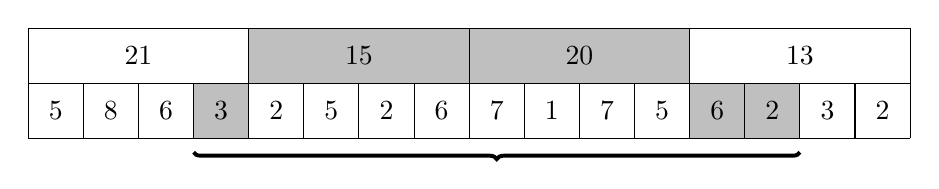
\begin{tikzpicture}[scale=0.7]
\fill[color=lightgray] (3,0) rectangle (4,1);
\fill[color=lightgray] (12,0) rectangle (13,1);
\fill[color=lightgray] (13,0) rectangle (14,1);
\draw (0,0) grid (16,1);

\fill[color=lightgray] (4,1) rectangle (8,2);
\fill[color=lightgray] (8,1) rectangle (12,2);
\draw (0,1) rectangle (4,2);
\draw (4,1) rectangle (8,2);
\draw (8,1) rectangle (12,2);
\draw (12,1) rectangle (16,2);

\node at (0.5, 0.5) {5};
\node at (1.5, 0.5) {8};
\node at (2.5, 0.5) {6};
\node at (3.5, 0.5) {3};
\node at (4.5, 0.5) {2};
\node at (5.5, 0.5) {5};
\node at (6.5, 0.5) {2};
\node at (7.5, 0.5) {6};
\node at (8.5, 0.5) {7};
\node at (9.5, 0.5) {1};
\node at (10.5, 0.5) {7};
\node at (11.5, 0.5) {5};
\node at (12.5, 0.5) {6};
\node at (13.5, 0.5) {2};
\node at (14.5, 0.5) {3};
\node at (15.5, 0.5) {2};

\node at (2, 1.5) {21};
\node at (6, 1.5) {15};
\node at (10, 1.5) {20};
\node at (14, 1.5) {13};

\draw [decoration={brace}, decorate, line width=0.5mm] (14,-0.25) -- (3,-0.25);

\end{tikzpicture}
\end{center}

Dado que el número de elementos individuales es $O(\sqrt n)$
y el número de bloques también es $O(\sqrt n)$,
la consulta de suma toma tiempo $O(\sqrt n)$.
El propósito del tamaño del bloque $\sqrt n$ es
que \emph{balancea} dos cosas:
el arreglo se divide en $\sqrt n$ bloques,
cada uno de los cuales contiene $\sqrt n$ elementos.

En la práctica, no es necesario usar el
valor exacto de $\sqrt n$ como parámetro,
y en su lugar podemos usar los parámetros $k$ y $n/k$ donde $k$ es
diferente de $\sqrt n$.
El parámetro óptimo depende del problema y de la entrada.
Por ejemplo, si un algoritmo a menudo recorre
los bloques pero rara vez inspecciona
elementos individuales dentro de los bloques,
puede ser una buena idea dividir el arreglo en
$k < \sqrt n$ bloques, cada uno de los cuales contiene $n/k > \sqrt n$
elementos.

\section{Combinación de algoritmos}

En esta sección discutimos dos algoritmos de raíz cuadrada
que se basan en combinar dos algoritmos en uno solo.
En ambos casos, podríamos usar cualquiera de los algoritmos
sin el otro y resolver el problema en tiempo $O(n^2)$.
Sin embargo, al combinar los algoritmos, el tiempo de ejecución
es solo $O(n \sqrt n)$.

\subsubsection{Procesamiento de casos}

Supongamos que tenemos una cuadrícula bidimensional
que contiene $n$ celdas.
A cada celda se le asigna una letra,
y nuestra tarea es encontrar dos celdas
con la misma letra cuya distancia sea mínima,
donde la distancia entre las celdas
$(x_1,y_1)$ y $(x_2,y_2)$ es $|x_1-x_2|+|y_1-y_2|$.
Por ejemplo, consideremos la siguiente cuadrícula:

\begin{center}
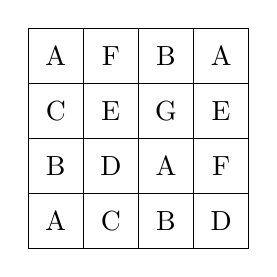
\begin{tikzpicture}[scale=0.7]
\node at (0.5,0.5) {A};
\node at (0.5,1.5) {B};
\node at (0.5,2.5) {C};
\node at (0.5,3.5) {A};
\node at (1.5,0.5) {C};
\node at (1.5,1.5) {D};
\node at (1.5,2.5) {E};
\node at (1.5,3.5) {F};
\node at (2.5,0.5) {B};
\node at (2.5,1.5) {A};
\node at (2.5,2.5) {G};
\node at (2.5,3.5) {B};
\node at (3.5,0.5) {D};
\node at (3.5,1.5) {F};
\node at (3.5,2.5) {E};
\node at (3.5,3.5) {A};
\draw (0,0) grid (4,4);
\end{tikzpicture}
\end{center}
En este caso, la distancia mínima es 2 entre las dos letras 'E'.

Podemos resolver el problema considerando cada letra por separado.
Con este enfoque, el nuevo problema es calcular
la distancia mínima
entre dos celdas con una letra \emph{fija} $c$.
Nos enfocamos en dos algoritmos para esto:

\emph{Algoritmo 1:} Recorrer todas las parejas de celdas con la letra $c$,
y calcular la distancia mínima entre tales celdas.
Esto tomará tiempo $O(k^2)$ donde $k$ es el número de celdas con la letra $c$.

\emph{Algoritmo 2:} Realizar una búsqueda en anchura que simultáneamente
comienza en cada celda con la letra $c$. La distancia mínima entre
dos celdas con la letra $c$ se calculará en tiempo $O(n)$.

Una forma de resolver el problema es elegir uno de los
algoritmos y usarlo para todas las letras.
Si usamos el Algoritmo 1, el tiempo de ejecución es $O(n^2)$,
porque todas las celdas pueden contener la misma letra,
y en este caso $k=n$.
También si usamos el Algoritmo 2, el tiempo de ejecución es $O(n^2)$,
porque todas las celdas pueden tener letras diferentes,
y en este caso se necesitan $n$ búsquedas.

Sin embargo, podemos \emph{combinar} los dos algoritmos y
usar diferentes algoritmos para diferentes letras
dependiendo de cuántas veces aparezca cada letra en la cuadrícula.
Supongamos que una letra $c$ aparece $k$ veces.
Si $k \le \sqrt n$, usamos el Algoritmo 1, y si $k > \sqrt n$,
usamos el Algoritmo 2.
Resulta que al hacer esto, el tiempo total de ejecución
del algoritmo es solo $O(n \sqrt n)$.

Primero, supongamos que usamos el Algoritmo 1 para una letra $c$.
Dado que $c$ aparece como máximo $\sqrt n$ veces en la cuadrícula,
comparamos cada celda con la letra $c$ $O(\sqrt n)$ veces
con otras celdas.
Por lo tanto, el tiempo utilizado para procesar todas esas celdas es $O(n \sqrt n)$.
Luego, supongamos que usamos el Algoritmo 2 para una letra $c$.
Hay como máximo $\sqrt n$ letras de este tipo,
por lo que procesar esas letras también lleva tiempo $O(n \sqrt n)$.

\subsubsection{Procesamiento por lotes}

Nuestro próximo problema también trata
una cuadrícula bidimensional que contiene $n$ celdas.
Inicialmente, cada celda excepto una es blanca.
Realizamos $n-1$ operaciones, cada una de las cuales primero
calcula la distancia mínima desde una celda blanca dada
hasta una celda negra, y luego pinta la celda blanca de negro.

Por ejemplo, consideremos la siguiente operación:

\begin{center}
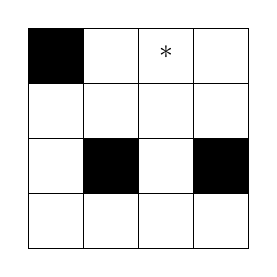
\begin{tikzpicture}[scale=0.7]
\fill[color=black] (1,1) rectangle (2,2);
\fill[color=black] (3,1) rectangle (4,2);
\fill[color=black] (0,3) rectangle (1,4);
\node at (2.5,3.5) {*};
\draw (0,0) grid (4,4);
\end{tikzpicture}
\end{center}

Primero calculamos la distancia mínima
desde la celda blanca marcada con * hasta una celda negra.
La distancia mínima es 2, porque podemos movernos
dos pasos a la izquierda hacia una celda negra.
Luego, pintamos la celda blanca de negro:

\begin{center}
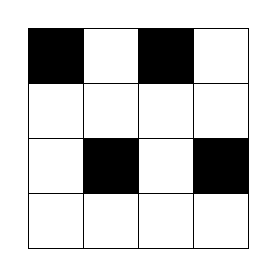
\begin{tikzpicture}[scale=0.7]
\fill[color=black] (1,1) rectangle (2,2);
\fill[color=black] (3,1) rectangle (4,2);
\fill[color=black] (0,3) rectangle (1,4);
\fill[color=black] (2,3) rectangle (3,4);
\draw (0,0) grid (4,4);
\end{tikzpicture}
\end{center}

Consideremos los siguientes dos algoritmos:

\emph{Algoritmo 1:} Usar búsqueda en anchura
para calcular para cada celda blanca la distancia a la celda negra más cercana.
Esto toma $O(n)$ tiempo, y después de la búsqueda,
podemos encontrar la distancia mínima desde cualquier celda blanca
a una celda negra en tiempo $O(1)$.

\emph{Algoritmo 2:} Mantener una lista de celdas que han sido
pintadas de negro, recorrer esta lista en cada operación
y luego agregar una nueva celda a la lista.
Una operación toma $O(k)$ tiempo donde $k$ es la longitud de la lista.

Combinamos los algoritmos anteriores dividiendo las operaciones en
$O(\sqrt n)$ \emph{lotes}, cada uno de los cuales consiste
en $O(\sqrt n)$ operaciones.
Al comienzo de cada lote,
realizamos el Algoritmo 1.
Luego, usamos el Algoritmo 2 para procesar las operaciones
en el lote.
Limpiamos la lista del Algoritmo 2 entre
los lotes.
En cada operación,
la distancia mínima a una celda negra
es la distancia calculada por el Algoritmo 1
o la distancia calculada por el Algoritmo 2.

El algoritmo resultante funciona en
tiempo $O(n \sqrt n)$.
Primero, el Algoritmo 1 se realiza $O(\sqrt n)$ veces,
y cada búsqueda funciona en tiempo $O(n)$.
Segundo, al usar el Algoritmo 2 en un lote,
la lista contiene $O(\sqrt n)$ celdas
(porque limpiamos la lista entre lotes)
y cada operación toma tiempo $O(\sqrt n)$.

\section{Particiones de enteros}

Algunos algoritmos de raíz cuadrada se basan en la siguiente observación:
si un entero positivo \( n \) se representa como una suma de enteros positivos,
tal suma siempre contiene a lo sumo \( O(\sqrt n) \) números \emph{distintos}.
La razón de esto es que para construir una suma que contenga el máximo número de números distintos, debemos elegir números \emph{pequeños}.
Si elegimos los números \( 1, 2, \ldots, k \),
la suma resultante es
\[
\frac{k(k+1)}{2}.
\]
Así, la cantidad máxima de números distintos es \( k = O(\sqrt n) \).
A continuación discutiremos dos problemas que pueden resolverse eficientemente usando esta observación.

\subsubsection{Mochila (Knapsack)}

Supongamos que tenemos una lista de pesos enteros cuya suma es \( n \).
Nuestra tarea es encontrar todas las sumas que pueden formarse usando un subconjunto de los pesos. Por ejemplo, si los pesos son \( \{1, 3, 3\} \), las sumas posibles son las siguientes:

\begin{itemize}[noitemsep]
\item \( 0 \) (conjunto vacío)
\item \( 1 \)
\item \( 3 \)
\item \( 1+3=4 \)
\item \( 3+3=6 \)
\item \( 1+3+3=7 \)
\end{itemize}

Usando el enfoque estándar de la mochila (ver Capítulo 7.4),
el problema puede resolverse de la siguiente manera:
definimos una función \( \texttt{possible}(x,k) \) cuyo valor es 1
si la suma \( x \) puede formarse usando los primeros \( k \) pesos,
y 0 en caso contrario.
Dado que la suma de los pesos es \( n \),
hay a lo sumo \( n \) pesos y
todos los valores de la función pueden calcularse
en tiempo \( O(n^2) \) utilizando programación dinámica.

Sin embargo, podemos hacer el algoritmo más eficiente
usando el hecho de que hay a lo sumo \( O(\sqrt n) \)
pesos \emph{distintos}.
Así, podemos procesar los pesos en grupos
que consisten en pesos similares.
Podemos procesar cada grupo
en tiempo \( O(n) \), lo que da lugar a un algoritmo de tiempo \( O(n \sqrt n) \).

La idea es usar un arreglo que registre las sumas de pesos
que pueden formarse usando los grupos procesados hasta ahora.
El arreglo contiene \( n \) elementos: el elemento \( k \) es 1 si la suma
\( k \) puede formarse y 0 en caso contrario.
Para procesar un grupo de pesos, recorremos el arreglo
de izquierda a derecha y registramos las nuevas sumas de pesos que
pueden formarse usando este grupo y los grupos anteriores.

\subsubsection{Construcción de cadenas}

Dada una cadena \( \texttt{s} \) de longitud \( n \)
y un conjunto de cadenas \( D \) cuya longitud total es \( m \),
consideremos el problema de contar la cantidad de formas
en que \( \texttt{s} \) puede formarse como una concatenación de cadenas en \( D \).
Por ejemplo,
si \( \texttt{s}=\texttt{ABAB} \) y
\( D=\{\texttt{A},\texttt{B},\texttt{AB}\} \),
hay 4 formas:

\begin{itemize}[noitemsep]
\item \( \texttt{A}+\texttt{B}+\texttt{A}+\texttt{B} \)
\item \( \texttt{AB}+\texttt{A}+\texttt{B} \)
\item \( \texttt{A}+\texttt{B}+\texttt{AB} \)
\item \( \texttt{AB}+\texttt{AB} \)
\end{itemize}

Podemos resolver el problema utilizando programación dinámica:
Sea \( \texttt{count}(k) \) el número de formas de construir el prefijo
\( \texttt{s}[0 \ldots k] \) usando las cadenas en \( D \).
Entonces \( \texttt{count}(n-1) \) da la respuesta al problema,
y podemos resolver el problema en tiempo \( O(n^2) \) usando una estructura de trie.

Sin embargo, podemos resolver el problema de manera más eficiente
usando el hashing de cadenas y el hecho de que hay a lo sumo \( O(\sqrt m) \)
longitudes de cadena distintas en \( D \).
Primero, construimos un conjunto \( H \) que contiene todos
los valores hash de las cadenas en \( D \).
Luego, al calcular un valor de \( \texttt{count}(k) \),
recorremos todos los valores de \( p \)
tales que hay una cadena de longitud \( p \) en \( D \),
calculamos el valor hash de \( \texttt{s}[k-p+1 \ldots k] \)
y verificamos si pertenece a \( H \).
Dado que hay a lo sumo \( O(\sqrt m) \) longitudes de cadena distintas,
esto resulta en un algoritmo cuyo tiempo de ejecución es \( O(n \sqrt m) \).

\section{Algoritmo de Mo}

\index{Algoritmo de Mo}

\key{El algoritmo de Mo}\footnote{Según \cite{cod15}, este algoritmo
lleva el nombre de Mo Tao, un programador competitivo chino, pero
la técnica ha aparecido anteriormente en la literatura \cite{ken06}.}
se puede usar en muchos problemas
que requieren procesar consultas de rango en
una matriz \emph{estática}, es decir, los valores de la matriz
no cambian entre las consultas.
En cada consulta, se nos da un rango \( [a,b] \),
y debemos calcular un valor basado en los
elementos de la matriz entre las posiciones \( a \) y \( b \).
Dado que la matriz es estática,
las consultas pueden procesarse en cualquier orden,
y el algoritmo de Mo
procesa las consultas en un orden especial que garantiza
que el algoritmo funcione eficientemente.

El algoritmo de Mo mantiene un \emph{rango activo}
de la matriz, y la respuesta a una consulta
sobre el rango activo se conoce en cada momento.
El algoritmo procesa las consultas una por una,
y siempre mueve los extremos del
rango activo insertando y eliminando elementos.
La complejidad temporal del algoritmo es
\( O(n \sqrt n f(n)) \) donde la matriz contiene
\( n \) elementos, hay \( n \) consultas
y cada inserción y eliminación de un elemento
toma tiempo \( O(f(n)) \).

El truco en el algoritmo de Mo es el orden
en que se procesan las consultas:
La matriz se divide en bloques de \( k=O(\sqrt n) \)
elementos, y una consulta \( [a_1,b_1] \)
se procesa antes que una consulta \( [a_2,b_2] \)
si cualquiera de las siguientes condiciones se cumple:
\begin{itemize}
\item \( \lfloor a_1/k \rfloor < \lfloor a_2/k \rfloor \) o
\item \( \lfloor a_1/k \rfloor = \lfloor a_2/k \rfloor \) y \( b_1 < b_2 \).
\end{itemize}

Así, todas las consultas cuyos extremos izquierdos están
en un cierto bloque se procesan una tras otra
ordenadas según sus extremos derechos.
Usando este orden, el algoritmo
realiza solo \( O(n \sqrt n) \) operaciones,
porque el extremo izquierdo se mueve
\( O(n) \) veces \( O(\sqrt n) \) pasos,
y el extremo derecho se mueve
\( O(\sqrt n) \) veces \( O(n) \) pasos. Por lo tanto, ambos
extremos se mueven un total de \( O(n \sqrt n) \) pasos durante el algoritmo.

\subsubsection*{Ejemplo}

Como ejemplo, consideremos un problema donde se nos dan un conjunto de consultas,
cada una correspondiente a un rango en un arreglo,
y nuestra tarea es calcular para cada consulta
el número de elementos \emph{distintos} en el rango.

En el algoritmo de Mo, las consultas siempre se ordenan de la misma manera, pero depende del problema cómo se mantiene la respuesta a la consulta.
En este problema, podemos mantener un arreglo \texttt{count} donde $\texttt{count}[x]$
indica cuántas veces aparece el elemento $x$
en el rango activo.

Cuando pasamos de una consulta a otra,
el rango activo cambia.
Por ejemplo, si el rango actual es
\begin{center}
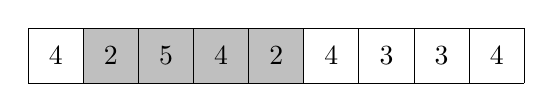
\begin{tikzpicture}[scale=0.7]
\fill[color=lightgray] (1,0) rectangle (5,1);
\draw (0,0) grid (9,1);
\node at (0.5, 0.5) {4};
\node at (1.5, 0.5) {2};
\node at (2.5, 0.5) {5};
\node at (3.5, 0.5) {4};
\node at (4.5, 0.5) {2};
\node at (5.5, 0.5) {4};
\node at (6.5, 0.5) {3};
\node at (7.5, 0.5) {3};
\node at (8.5, 0.5) {4};
\end{tikzpicture}
\end{center}
y el siguiente rango es
\begin{center}
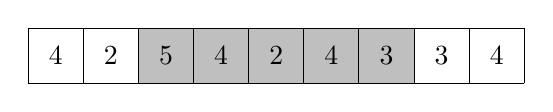
\begin{tikzpicture}[scale=0.7]
\fill[color=lightgray] (2,0) rectangle (7,1);
\draw (0,0) grid (9,1);
\node at (0.5, 0.5) {4};
\node at (1.5, 0.5) {2};
\node at (2.5, 0.5) {5};
\node at (3.5, 0.5) {4};
\node at (4.5, 0.5) {2};
\node at (5.5, 0.5) {4};
\node at (6.5, 0.5) {3};
\node at (7.5, 0.5) {3};
\node at (8.5, 0.5) {4};
\end{tikzpicture}
\end{center}
habrá tres pasos:
el extremo izquierdo se mueve un paso a la derecha,
y el extremo derecho se mueve dos pasos a la derecha.

Después de cada paso, el arreglo \texttt{count}
necesita ser actualizado.
Después de agregar un elemento $x$,
aumentamos el valor de 
$\texttt{count}[x]$ en 1,
y si $\texttt{count}[x]=1$ después de esto,
también aumentamos la respuesta a la consulta en 1.
De manera similar, después de eliminar un elemento $x$,
disminuimos el valor de 
$\texttt{count}[x]$ en 1,
y si $\texttt{count}[x]=0$ después de esto,
también disminuimos la respuesta a la consulta en 1.

En este problema, el tiempo necesario para realizar
cada paso es $O(1)$, por lo que la complejidad temporal
total del algoritmo es $O(n \sqrt n)$.